\pdfoutput=1 
\documentclass[12pt,a4paper]{report}
\usepackage{cite}
\usepackage{calligra}

\usepackage{xcolor}
\definecolor{darkPurple}{HTML}{3333B2}
\definecolor{forestGreen}{HTML}{337700}
\definecolor{shadecolor}{HTML}{CCCCCC}
\definecolor{darkGrey}{HTML}{4E4F86}
\definecolor{Crimson}{HTML}{DC143C}
\definecolor{transparentBlue}{HTML}{EBEBF8}
\usepackage{hyperref}
\hypersetup{colorlinks=true, linkcolor=darkPurple, citecolor=darkPurple}
\usepackage[pdftex]{graphicx}
\graphicspath{{./figures/}}
\usepackage[cmex10]{amsmath}
\usepackage{amssymb}
\usepackage{multirow}	
\usepackage[]{subfig}
\usepackage[toc]{appendix}
\usepackage{listings}
\usepackage[english]{babel}
\usepackage{fancyvrb}

\lstset { %
  language=C,
  backgroundcolor=\color{black!5}, % set backgroundcolor
  basicstyle=\footnotesize,        % the size of the fonts that are used for the code
  commentstyle=\color{forestGreen},    % comment style
  keywordstyle=\color{blue},       % keyword style
  keepspaces=true,                 % keeps spaces in text, useful for keeping indentation of code (possibly needs columns=flexible)
  showspaces=false,
  showstringspaces=false
}
% Font settings to get IEEE-style fonts
%\renewcommand{\sfdefault}{phv}
%\renewcommand{\rmdefault}{ptm}
%\renewcommand{\ttdefault}{pcr}

\title{
{\Huge Sitar}\\
{\Large Simulation Tool for Architectural Research}\\
{\small Version 2.0}\\[2em]
{\large User Manual and Technical Document}
}
\author{
{\small Neha V. Karanjkar \qquad Madhav P. Desai}\\
{\small Department of Electrical Engineering}\\
{\small Indian Institute of Technology Bombay}\\[1em]
{\small Revision: April 2017}\\[1em]

\includegraphics[width=5em]{iitblogo.pdf}
}
\date{}
\begin{document}
\maketitle

\tableofcontents
\chapter{Introduction}


Sitar is a framework for modeling discrete-event, discrete-time systems.  It
consists of a simulation kernel and a language for describing the system to be
modeled.  Descriptions written in this language get translated to C++ code and
can be compiled to get a simulation executable.


A system can be described as a set of {\em modules} (which are behavioral
entities in the system) communicating over channels called {\em nets}.
All modules run concurrently on a global clock. 
%
The language provides a means for describing the system structure (as an
interconnection of modules) in a hierarchical and modular way.  The behavior of
each module can be described in an imperative manner as a {\em sequence} of
statements. The statements include conditional and unconditional time-delays,
branch and loop constructs, parallel blocks and instantaneous code blocks. In
addition, C++ code can be embedded into a module description in a
straightforward and well-defined manner.  
%
The sitar language parser/translator has been built using Antlr V3\cite{Antlr}.
It translates each module description into a C++ class.
The generated classes inherit methods from the simulation kernel
to allow execution of their behavior. 

The simulation kernel is cycle-based and uses a two-phase execution
algorithm. In this algorithm, each clock cycle is divided into two
phases: {\em phase 0} and {\em phase 1}. All input actions by modules
are restricted to phase 0 and all output actions are restricted to phase 1. 
Thus there is a minimum delay of a single cycle for information to
propagate from one module to another. Combinational loops, if present,
must lie entirely within a module. This restriction makes the
simulation algorithm simple and easy to parallelize. 
%
The sitar kernel has been parallelized using OpenMP\cite{OpenMP}.
Individual modules or a group of modules can be mapped to separate
OpenMP threads that synchronize at the end of each phase.


The sitar framework includes systematic support for logging.
The logging mechanism uses C++'s {\tt std::ostream} library. Individual modules 
can send their logs to a common stream or separate streams. The logging
can be enabled/disabled at compile-time or run-time, and run-time
logging behavior can be controlled individually for each module.

The generated C++ models can be easily connected to
existing models (such as processor front-ends) 
for co-simulation using direct function calls or through
inter-process communication. This makes the framework ideally
suited for computer architectural studies.

In this document, we first present the basic execution model 
used by sitar in Chapter \ref{chap:execution_model}.
In Chapter \ref{chap:language} we describe the sitar language
using illustrative examples. The language syntax is available in 
EBNF format as a separate hyperlinked document named {\tt sitar\_syntax.xhtml}.
In Chapter \ref{chap:translation_scheme} we present the scheme used for 
translating constructs such as time-delays and parallel blocks
in sitar to C++ code.

\newpage
\section{Getting Started}
Sitar is written for Linux. 
It is available as open-source with an MIT licence at \cite{SitarGit}. 
Installation instructions are present in the file {\tt INSTALL} and 
several examples are present in the {\tt examples/} folder.
The following is a simple example of a sitar description. The system
consists of a single module that simply prints \lq\lq Hello World\rq\rq\.
after a delay of one cycle.

\begin{itemize}
\item[] 
\begin{Verbatim}[frame=single]
module Top
    behavior
        wait (1,0);
        $std::cout<<"Hello World";$ ;
        stop simulation;
    end behavior
end module
\end{Verbatim}

\item The language is case-sensitive
\item The system description must include the definition 
of a single module named {\tt Top}. This represents the 
top-level module in the system hierarchy, and is instantiated
at the start of simulation. All other components in the system 
must be contained within this module.
\item A module may have a behavior block. The behavior block
consists of a {\em sequence} of statements, separated by the
sequence operator (a semi-colon). In the above example,
the behavior consists of three statements:

 \begin{enumerate}
 \item A wait statement that produces a delay of one cycle.
 \item A C++ code block delimited by \$ symbols. Contents of a code-block
 are pasted verbatim in the generated C++ code.
 \item A statement to stop the simulation when control reaches here.
 \end{enumerate}
 \item To simulate this example, save it as a file named (say) {\tt Hello.sitar}.
Then run the translator and compiler using commands:
\begin{Verbatim}[frame=single]
$ sitar translate Hello.sitar
$ sitar compile -o Hello
\end{Verbatim}
This produces a single simulation executable named {\tt Hello}. Run the executable
to obtain the simulation results.
\end{itemize} 



\chapter{Execution Model} \label{chap:execution_model}

The basic components in a sitar system are {\em modules} and {\em nets}.
Modules are behavioral entities in the system and 
nets are channels of communication between them.
Figure \ref{fig:ExecutionModel} illustrates a system 
with four modules contained inside the Top module.
%
All modules run concurrently on a single clock.  A module can communicate with
another module via transfer of {\em data tokens} (which are packets of
information) over a net connecting the two modules.  Each net provides a fixed
amount of FIFO buffering for data tokens. Nets are passive components, and
their state can change only upon input or output actions by modules.
%
A module's interface to a net is called a {\em port}. 
A port can either be an {\em inport} or an {\em outport}.
Each net is connected to exactly one inport and one outport.
%
\begin{figure}[h]
\centering
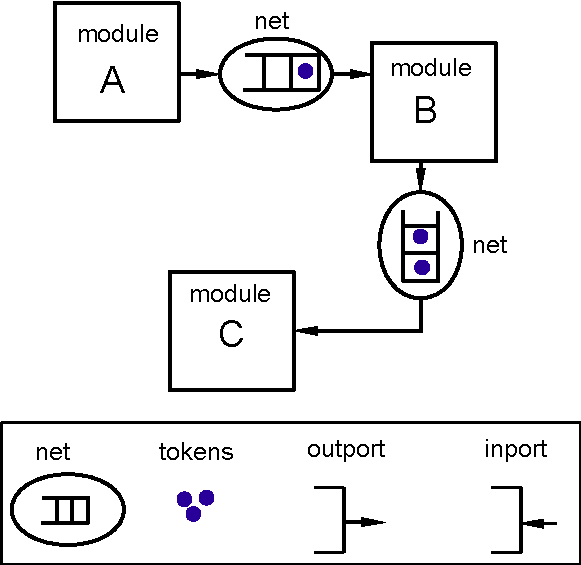
\includegraphics[width=0.8\textwidth]{ExecutionModel.pdf}
\caption{Example of a system in sitar}
\label{fig:ExecutionModel}
\end{figure}
\\

Simulation is cycle-based and uses a two-phase execution algorithm.
In this algorithm, each clock cycle is divided into two phases : {\em phase 0}
and {\em phase 1}. A module is allowed to input tokens from a net in 
phase 0 only, and output tokens to a net in phase 1 only. 
Thus the state-updation of a net is race-free.
As a consequence, the propagation of information from one
module to another incurs a delay of at-least one clock cycle.
The framework can thus model any system that can be
described as interconnected Moore machines.
%
This restriction leads to a simple simulation algorithm
that is easily parallelized. In this simulation algorithm, 
in each phase, the behavior of each module in the system is executed exactly once.
The result does not depend on the order of execution among modules.
The simulation algorithm is as follows:

\begin{verbatim}
cycle = 0
while (cycle < total_simulation_cycles)
{
   phase=0
   for each module m :
        m.run(cycle,phase)
   phase=1
   for each module m :
        m.run(cycle,phase)

   cycle=cycle+1
}
\end{verbatim}

Within a phase, modules can be executed independently of each other.
Thus the execution of individual modules can be mapped to 
separate threads running concurrently and synchronizing at the end of each phase.




\chapter{System Description Language} \label{chap:language}

This chapter presents the sitar system description language
along with several illustrative examples.

\section{Lexical Aspects}

\begin{itemize}
\item The language is case-sensitive

\item C++ style single-line comments are supported. A comment starts with {\tt//} 
and extends till the end of the line. Comments are 
ignored during translation.

\item C++ code can be embedded within a sitar description as
a code block. A code block is delimited by {\tt \$} symbols, and its contents
are inserted verbatim into the translated C++ code.

\item Sitar identifiers (such as module names) must begin with a letter from the alphabet, and can contain 
any number of letters, digits or underscores.

\item The list of keywords used by the language is listed in Section \ref{sec:keywords}. 
The precise syntax is available in EBNF form as a separate document
({\tt sitar\_syntax.xhtml}).
\end{itemize}


\section{Basic Design Units}

The basic design units in a sitar description are {\em modules} and {\em procedures}. 
Modules are structural elements that can be instantiated independently, 
whereas a procedure describes a sequence of actions
that can be invoked by a module or from within another procedure.
A design unit can be defined once and instantiated multiple times.
The following example contains two design units: an empty module named {\tt Foo}
and a procedure named {\tt Bar} that does nothing.
\begin{Verbatim}[frame=single]
module Foo
end module

procedure Bar
	behavior
		nothing;
	end behavior
end procedure
\end{Verbatim}

\begin{itemize}
\item A design unit must lie entirely
within a file, but a single file can contain multiple design units.

\item A system description can span multiple files. The translator
needs to be run on each file individually and the generated C++ code
can be compiled together to get a single executable.
\end{itemize}

There are two aspects to a sitar description:
\begin{itemize}
	\item Structure of the system: how modules are interconnected
	\item Behavior of each module
\end{itemize}
We describe each of these aspects next.


\section {Describing Structure}
	The structural aspects of a system description include information such as
	how modules are interconnected using nets, and attributes such as 
	capacities of nets and widths of ports (to model communication bandwidth).
	The language supports the following features:
	\begin{itemize}
	\item Hierarchy: modules can contain other modules. There is no limit 
	to the depth to which modules can be nested.
	\item Generation of regular structures such as arrays of modules and nets
	and their connections in a regular pattern is supported by the language.
	1 and 2 dimensional arrays of nets, ports and modules are supported.
	\item Generics: modules can be parametrized
	\end{itemize}

	Elaboration begins by instantiating a single module.  \textbf{By
	convention, this top-level module in the hierarchy has to be named
	\texttt{Top}}.  Thus, if the system to be simulated has multiple
	modules, they have to be enclosed inside a single module named \texttt{Top}.\\

	A module can have the following components:
	\begin{itemize}
	\item A declaration of module parameters
	\item Ports: a port can either be an input-port or an output port.
	Ports have a \emph{width} attribute.
	\item A declaration of instances of submodules contained within this module, along with their types.
	\item A declaration of nets within the module. Nets have a \emph{capacity} attribute.
	\item Connections between nets and ports of submodules.
	\item A behavior block -  describing the local behavior of the module
	\end{itemize}
	
	Note that:
	{\renewcommand{\labelitemi}{$\triangleright$}
	\begin{itemize}
	\item Data tokens placed in nets have a \emph{weight} attribute. 
	\item \emph{Weight}, \emph{capacity}, and \emph{width} attributes can have non-negative integer values.
	\item \emph{Capacity} of a net represents the maximum 
	sum of weights of data tokens that can be stored in a net at any given time.
	\item \emph{Width} of a port represents the maximum sum of weights of data tokens that can pass across
	a port in a single cycle.
	\end{itemize}}



\item The system can be described in a hierarchical manner, 
with modules containing instances of other modules.  
The description must always contain a single module named
{\tt Top} which represents the top-level module in the structural
hierarchy, and contains all other modules in the system.  
This top-level module is instantiated at the start of simulation.






\begin{itemize}
\item Tokens have a {\tt width} parameter, which represents the
number of bytes of data that are carried by the token.

\item A net has two parameters:
{\tt width} and {\tt capacity}. A net with width $W$ can only 
contain tokens of width $W$. The capacity of a net is the maximum number
of tokens it can contain at a time.

\item Ports have a single parameter {\tt width}. A port with width $W$ can only be 
connected to a net of width $W$.
\end{itemize}

	\section{Overview}
	This chapter describes how a system can be described using the SiTAR
	language, and gives the semantics of behavioral statements.
	Constructs in the language are explained using examples. Formal syntax is 
	given in the next chapter.\\

	A system consists of modules interconnected using nets. 
	System description consists of the following aspects:
	\begin{itemize}
	\item Structure of the system: how modules are interconnected
	\item Local behavior of each module
	\item Global behavior (tasks) in the system, and information about when they are triggered
	\end{itemize}
	The third aspect of the description (tasks) is optional.  SiTAR
	provides a language for describing the first two aspects, while global
	tasks currently have to be described as C++ code derived from a set of
	base classes provided to the user.  In addition, the user can describe
	parts of functionality directly as C++ code which can be embedded in a
	well defined manner into the system description.\\

	
	A system description  can span multiple files. The translator has to be
	run on each of these files individually, and the translated code can be compiled together
	to get a simulation executable.
	The basic design units in a SiTAR description are \textbf{procedures} and \textbf{modules}.
	A design unit can be described once and instantiated multiple times.
	Modules are structural elements that can be instantiated independently, 
	whereas a procedure describes a part of local behavior of a module, 
	and needs to be instantiated \emph{inside} some module, or another procedure.
	The following section handles each of the 3 aspects of system description one-by-one.\\

	\section{Describing Structure}
	
	The structural aspects of a system description include information such as
	how modules are interconnected using nets, and attributes such as 
	capacities of nets and widths of ports (to model communication bandwidth).
	The language supports the following features:
	\begin{itemize}
	\item Hierarchy: modules can contain other modules. There is no limit 
	to the depth to which modules can be nested.
	\item Generation of regular structures such as arrays of modules and nets
	and their connections in a regular pattern is supported by the language.
	1 and 2 dimensional arrays of nets, ports and modules are supported.
	\item Generics: modules can be parametrized
	\end{itemize}

	Elaboration begins by instantiating a single module.  \textbf{By
	convention, this top-level module in the hierarchy has to be named
	\texttt{Top}}.  Thus, if the system to be simulated has multiple
	modules, they have to be enclosed inside a single module named \texttt{Top}.\\

	A module can have the following components:
	\begin{itemize}
	\item A declaration of module parameters
	\item Ports: a port can either be an input-port or an output port.
	Ports have a \emph{width} attribute.
	\item A declaration of instances of submodules contained within this module, along with their types.
	\item A declaration of nets within the module. Nets have a \emph{capacity} attribute.
	\item Connections between nets and ports of submodules.
	\item A behavior block -  describing the local behavior of the module
	\end{itemize}
	
	Note that:
	{\renewcommand{\labelitemi}{$\triangleright$}
	\begin{itemize}
	\item Data tokens placed in nets have a \emph{weight} attribute. 
	\item \emph{Weight}, \emph{capacity}, and \emph{width} attributes can have non-negative integer values.
	\item \emph{Capacity} of a net represents the maximum 
	sum of weights of data tokens that can be stored in a net at any given time.
	\item \emph{Width} of a port represents the maximum sum of weights of data tokens that can pass across
	a port in a single cycle.
	\end{itemize}}
	\subsection{Example}
	Following is a simple example of a shift register, with a parametrizable number of stages:
	\begin{verbatim}
        //Shift register consists of a
        //producer, connected to a consumer through 
        //an array of shift register stages.
        //The number of stages and delay of 
        //each stage is parametrizable.

        module Top
                submodule S : ShiftRegister<2,1> 
                //Instantiate a shift register with 2 stages,
                //each stage having delay=1
        end module


        module ShiftRegister 
                parameter int N = 2  //number of stages
                parameter int DELAY = 1 //delay of each stage
                
                submodule P : Producer
                submodule C : Consumer
                submodule_array stage[N]  : Stage<DELAY>
                net_array n[N+1] : capacity 1

                //make connections
                for i in 0 to (N - 1)
                        stage[i].pin <= n[i]
                        stage[i].pout => n[i+1]
                end for
                P.pout => n[0]
                C.pin <= n[N]
        end module
                        

        module Stage
                parameter int DELAY = 1  //delay of each stage
                inport pin         : width 1
                outport pout       : width 1
                
                behavior 
                //<....describe behavior here....>
                end behavior
        end module

	\end{verbatim}

\section{Keywords}\label{sec:keywords}
The following is a list of keywords used by the language:
	
	
	\begin{itemize}
	
	\item module
	\item procedure
	\item behavior
	\item end
	\item parameter
	\item int
	\item bool
	\item char
	
	\item[] Keywords for declaring structural components:
	
	\item inport
	\item inport\_array
	\item outport
	\item outport\_array
	\item net
	\item net\_array
	\item submodule
	\item submodule\_array
	\item width
	\item capacity
	\item for
	\item in
	\item to
	
	\item[] Keywords used by behavioral statements:
	\item wait
	\item until
	\item if
	\item then
	\item else
	\item do
	\item while
	\item nothing
	\item run
	\item stop
	\item simulation
	\item log
	\item or
	\item and
	\item not
	
	\item[]Reserved variable names within a module or procedure:
	\item this\_cycle	
	\item this\_phase
	\item current\_time
	\item parent
	\end{itemize}
	

	\section{Embedding C++ code}
	Each module gets translated into a C++ class,
	derived from a base class.
	C++ code delimited by the dollar signs can be embedded at several places in the 
	description using code blocks. Code blocks are of 4 
	types, depending on where the user-code gets inserted in
	the translated code:
	\begin{enumerate}
		\item \emph{Include block}:  contents are inserted at the top of the header file, useful for including
		header files in the generated code.
		\item \emph{Declaration block}: contents are inserted in the body of the class in the header file
		\item \emph{Initialization block}: contents are inserted inside the constructor for the class
		\item \emph{Code block statement}: the contents become part of a single behavioral statement.
		A code block statement can only exist within a behavior block. The other 3 can occur anywhere inside
		the module body, or within the behavior block.
	\end{enumerate}
	Following example demonstrates code inclusion in a single module. 2 variables are declared, initialized,
	and their value is modified and printed from within a behavior block:
    \begin{verbatim}
    //various ways of C++ code embedding
    module CodeBlocks
        decl $int x,y,z;$ 
        //goes into class body (private data members of class)
        
        init $x=10;y=20;$ 
        //goes into module class' constructor
        
        include $#include<iostream>$ 
        //goes into header section

    behavior 

        nothing;
        decl $int a;$; 
        //include, decl and init blocks can also be placed 
        //inside the behavior block
        init $z=30;$;
        $cout<<"\n"<<x<<y<<z;$; //becomes a behavioral statement
        nothing;
        do nothing while($(1==2)$) end do; 
        //expression between dollar signs gets copied 
        //as-is in the translated C++ code
    end behavior
    end module

     \end{verbatim}


	




	\section{Describing Local Behavior}
	A module can optionally have a behavior block. 
	The behavior block consists of a single thread of execution
	which can have loops, can fork into parallel branches,
	and have time delays. The imperative language is
	inspired from Esterel\cite{esterel}.
	This section describes the constructs in the behavior block
	and explains their semantics.\\

	\subsection{Execution of the Behavior block}
	In each phase of simulation, the behavior block
	of every module is executed once (as listed in section \ref{subsec:implementedAlgorithm}).
	Every module has a \emph{state}. This state comprises values of all variables and
	constants declared by the user, and some state holders that are
	inferred implicitly from the description.  Execution of a behavior block
	corresponds to executing a \emph{sequence} of statements which operate
	on this state. In each phase of simulation, this sequence is executed
	until it terminates, or converges for the current phase.\\

	\subsection{Sequence}
	A sequence is an ordered set of statements.
	Some type of statements can in-turn contain sequences.
	Thus the description may contain several nested sequences. 
	Each sequence that occurs in the description is associated with a pointer, 
	which remembers the currently active statement in that sequence.\\


	After executing a sequence, it can have 
	one of the following as its \emph{status}:
	\begin{itemize}
	\item Converged: the sequence is active, but has converged for the current phase
	\item Terminated: the sequence has finished executing
	\end{itemize}


	Consider a sequence $Q$ with statements
	$\{S_1,S_2,...S_n\}$. Let $i$ be a pointer that points 
	to the currently active statement $S_i$.\\


	Execution of a sequence within a single phase can be described as follows:\\

	%\begin{algorithmic}
	%\If {the sequence has terminated}
	%	\State{do nothing; \textbf{exit}}
	%\Else 
	%	\Loop
	%		\State{execute $S_i$}
	%		\If {$S_i$ converges}
	%			\State {$Q$ converges; \textbf{exit}}
	%		\ElsIf {$S_i$ terminates and $i=n$}
	%			\State{ $Q$ terminates; \textbf{exit}}
	%		\ElsIf { $S_i$ terminates and $i<n$}
	%			\State {$i \gets i+1$}
	%		\EndIf
	%	\EndLoop
	%\EndIf
	%\end{algorithmic}



	\subsection{Statement}
	Statements could be atomic, or compound (in-turn containing sequences of statements).
	When a statement is executed, it can either terminate instantaneously,
	or converge, and remain active for the next phase.
	Following is the syntax and behavior of each type of statement:\\

	\subsection{Code block statement}
		\texttt{\$}\\
		\textit{C++ statements}\\
		\texttt{\$}\\

	The C++ code contained inside the code delimiters is executed 
	as a single behavior block statement, and finishes instantaneously.


	\subsection{Function call statement}
		\textit{identifier} \texttt{(}\textit{argument\_ list} \texttt{)}\\

	It is assumed that a C++ function with the same name as \textit{identifier}
	has been defined, and made visible to the module class. All
	functions are assumed to return void.
	Argument list is a comma-separated list of constants and identifiers.
	If the user wishes the function to modify values of variables, they can
	be passed to the function as reference arguments.
	The C++ function-call is treated as a single behavior block statement 
	and finishes instantaneously.


	\subsection{Variable assignment statement}
		\textit{identifier} \texttt{=} \textit{expression}\\

	Expression is evaluated, and its value is assigned to the variable on the left.
	The statement terminates instantaneously.


	\subsection{Nothing statement}
		\texttt{nothing}\\

	A nothing statement terminates instantaneously.

	\subsection{Logging statement}
		\texttt{log} \textit{string}\\
	Sends \textit{string} to core logger. If logging is enabled,
	the string gets printed into the log stream.

	\subsection{Wait statement}
	Wait statements are the only statements that can produce delays.
	There are 3 types of wait statements:


	\subsubsection{wait(e1,e2)}

	Waits for a finite time(e1,e2), where e1 and e2 are expressions whose values correspond to 
	number of cycles and number of phases, respectively.\\


	If e1 and e2 are non-constant expressions, their values are evaluated only \emph{once} 
	when the statement is activated, and remembered for successive phases for which the 
	statement remains active. When executed, the statement returns status \emph{converged}
	if the delay has not elapsed in the current phase, and \emph{terminated} otherwise.\\


	For example, \texttt{wait(0,0)} terminates instantaneously. 
	A \texttt{wait(1,1)}, when executed at time(0,0) has status \emph{converged}
	upto time(1,0) and terminates at time (1,1).


	\subsubsection{wait until (expression)}

	This statement waits until the given expression evaluates to \emph{true}.\\

	The expression is evaluated \emph{each} time the statement is executed. If the value is non-zero,
	the statement terminates, else remains converged until the next phase, when the statement is executed again.

	For example, \texttt{wait until (1)} terminates instantaneously, and \texttt{wait until (v1==0)}
	terminates when the value of a variable v1 becomes zero.



	\subsubsection{wait}
	A simple wait is equivalent to wait(0,1) and pauses for one phase.

	
	
	
	
	\subsection{Stop statement}
	Stop statements are used to stop simulation from within the
	behavior block. There are 2 kinds of stop statements: 
	\texttt{stop module} and \texttt{stop simulation}.

	\subsubsection{stop module}
	Stops the execution of the module in which
	this statement occurs, and all the modules contained within it,
	starting from the \emph{next phase} of simulation. All behavior in the
	current phase is executed until convergence.
	Stop statement is instantaneous.\\
	Example:
	\begin{verbatim}
	behavior 
		wait(1,0);
		stop module;
		$std::cout<<"\nHello";$ ;
		wait(0,1);
		$std::cout<<" World"; $ ;
	end behavior
	\end{verbatim}
	This behavior will cause \texttt{Hello} to be printed before simulation
	stops, as the \texttt{stop module} statement finishes instantaneously,
	and control goes to the code block statement which is executed in the
	same phase.  Simulation of this module stops from time \texttt{(1,1)}
	onwards.  Behavior of the system up till time \texttt{(1,0)} is
	executed until convergence.
	
	
	\subsubsection{stop simulation}
	Stops entire simulation . All behavior
	is executed till convergence for the current phase, and the 
	simulation stops from next phase onwards. This is equivalent to  
	a \texttt{stop module} statement executed by the \texttt{Top} module.

	
	\subsection{Run procedure statement}
		\texttt{run} \textit{procedure\_instance\_name}\\

	The \texttt{run procedure} statement is a compound statement.
	A procedure in turn consists of a sequence of statements.
	The statement immediately activates the sequence contained inside
	the procedure. If the sequence inside the procedure converges,
	the run statement converges. If the procedure terminates, 
	the run statement terminates. Each run statement 
	occurring in a behavior block should refer to a unique procedure instance,
	as a procedure instance stores the state of the sequence.
	Procedures, and their use is described in detail in section \ref{sec:procedures}.


	\subsection{If-else statement}
	\texttt{if}  \textit{expression\_b} \texttt{then}\\
	\hspace{1 cm}\textit{sequence\_s1}\\
	( \texttt{else}\\
	\hspace{1 cm}\textit{sequence\_s2})? \\
	\texttt{end if}\\
	
	
	The \textit{if statement} is a compound statement, and contains two sequences \textit{s1} and {s2}.
	The expression is evaluated \emph{once}, immediately when the if-statement is activated. 
	If the expression evaluates to a non-zero value, branch s1 is activated, else branch s2 is activated.
	The statement converges if the active branch converges, and terminates, if the active branch terminates.\\

	For example,
	\begin{verbatim}
	if(v1<10) then
		wait(10,0)
	else
		wait(20,0)
	end if
	\end{verbatim}
	waits for 10 cycles, if the value of a variable 
	v1 is less than 10 at the instant the statement 
	is first activated, and waits for 20 cycles 
	otherwise.

	\subsection{Do-while statement}
		\texttt{do}\\
		\ \textit{sequence\_s1}\\
		\texttt{while} \textit{expression\_b} \texttt{end do}\\

	The sequence s1 is immediately activated when the do-while statement begins.
	If s1 converges, the do-while statement converges too. If s1 terminates, the expression is evaluated,
	and, if it returns a non-zero value, s1 is activated again. If the expression returns zero, 
	the do-while statement terminates.\\

	If there is no delay in s1, and if the value of expression does not become zero within s1,
	a loop can execute forever. The user can set an upper bound to the number of loop iterations
	that are allowed to execute in a single phase. If this limit is crossed, a runtime error is thrown.\\

	Example,

	\begin{verbatim}
	count=0;
	do
		wait;
		doStuff(v1);
		count=count+1;        
	while (count<10 and v1!=0) end do
	\end{verbatim}

	This code executes doStuff(v1) at-most 10 times, once every phase, 
	until v1 becomes zero.


	\subsection{Parallel block}
		\texttt{[} \textit{sequence} ( \texttt{$\parallel$} \textit{sequence} )+ \texttt{]}\\

	A parallel statement executes all of the sequences contained in it, in parallel.\\

	When a parallel statement is activated, all its child sequences are immediately activated.
	All the active branches are executed till convergence. 
	A parallel statement terminates if all its branches terminate.
	If at-least one branch does not terminate, but converges, 
	the parallel statement converges.\\

	Changes made to the behavior block state by one branch are immediately visible 
	to all the other active branches.\\

	Consider the following example:
	\begin{verbatim}
	v1=0;
	v2=0;
	[wait; v1=1; wait until (v2==1) || wait until (v1==1); v2=1; wait]
	\end{verbatim}

	When the parallel statement begins, nothing happens for the first phase.
	In the second phase, branch 1 sets a variable v1. 
	Branch 2, which is waiting for v1 to be set, 
	immediately sees the updated value of v1, 
	and updates v2 to 1 in the same phase. 
	Branch 1, waiting for v2==1 terminates.
	In the third phase, branch 2 terminates, 
	and the whole parallel statement finishes.
	
	
	
	
	\section{Procedures}\label{sec:procedures}
	
	\textit{Procedures} in SiTAR are akin to functions in C or C++. 
	A procedure is a sequence of behavioral statements which can be 
	described once, and invoked at multiple places in a SiTAR
	description. They provide re-usability in description. 
	In addition:
	\begin{itemize}
	\item There is a means to transfer information to and from a procedure.
	(In C or C++, this is achieved through function arguments and return values)
	\item A procedure can have local variables.
	\item Nesting procedures is possible. A procedure can
	in-turn call another procedure. (\textbf{Note:} Recursion is
	currently not supported. However, it is possible to add this in a
	future version of the language if needed.)
	\end{itemize}

	


	\subsection{Describing a Procedure}
	Modules and procedures are the basic design units in SiTAR. A procedure definition 
	is similar to a module definition, except the following differences:
	\begin{enumerate}
	\item a procedure \emph{must} have a behavior block
	\item a procedure cannot have any structural components (such as sub-modules, nets and ports)
	\item procedures must be invoked from within a behavior block of a module or another procedure.
	\end{enumerate}
	A procedure can have local variables (declared by using code blocks ),
	and also have sub-procedures. A procedure can be global, or local to a module. 
	Section \ref{sec:ProcedureSyntax} gives the syntax for a procedure definition.
	Following is an example of a simple procedure description that waits 2 cycles 
	and prints \texttt{Hello World}, and updates the value of its local variable \texttt{a}:
\begin{verbatim}
 procedure Foo
         //declare and initialize local variables
         $decl  int a;  $enddecl;
         $init  a=0;    $endinit

         behavior 
             wait (2,0);
             $std::cout<<"\nHello World";$ ;
             a=3;
         end behavior
 end procedure
\end{verbatim}


	\subsection{Invoking a Procedure}
	\textbf{Note:} A procedure can be called by a module \emph{as well as} another
	procedure.  In the following discussion, for clarity, the module or the
	procedure \emph{calling} a procedure is referred to as the
	\emph{parent}, and the procedure being \emph{called} is referred to,
	simply as the \emph{procedure}.\\

	A procedure definition gets translated to a C++ class, and 
	each invocation of a procedure becomes an object of this class. 
	This object stores the \emph{state} of the procedure call.
	The parent that wishes to call a procedure 
	must first declare objects of the Procedure-class' type as its
	data-members.

	Following is an example of a module calling the procedure \texttt{Foo}
	defined in the previous section.
\begin{verbatim}
module A
        //declare two procedure instances of type Foo
        procedure f1,f2 : Foo

        behavior 
                ... behavioral statements...;
                run f1;
                ...
                [run f1 || run f2];
                ...
        end behavior
end module
\end{verbatim}
	The instances \texttt{f1} and \texttt{f2} become data-members
	of class A.	
	A single procedure instance can be invoked safely multiple times in a
	behavior block, if it is known that any two invocations can never be
	active simultaneously.  If two invocations of a single procedure
	instance are active at the same time (by being within different branches
	of a parallel block), the behavior is undefined.
	In such a case separate procedure instances should be used.


	\subsection{Passing Information}
	Information can be passed between the parent and the procedure instance
	in two ways:
	\begin{enumerate}
	\item The parent can access public data-members or methods 
	in the procedure instance.  This is possible as the procedure instance is a named
	data-member of the parent class.  Consider the example:
	\begin{verbatim}
module A
        //declare two procedure instances of type Foo
        procedure f1,f2 : Foo

        behavior 
                ... behavioral statements...;
                //modify local variables of f1
                
				$f1.a=10; $;

                run f1;
                
				...
                //read local variables of f1
                if(f1.a==0) then ... end if;
                ...
        end behavior
end module
\end{verbatim}
	\item The procedure instance can access public data-members or methods of
	its parent. This is possible by having every procedure instance store a 
	pointer to its parent. This pointer is named \texttt{parent} and is initialized
	at elaboration time. Depending on the type (class) of the parent pointer, there
	are two types of procedures: \emph{global} and \emph{local}, described in the next
	section.
	\end{enumerate}

	\subsection{Local and Global Procedures}
	\begin{description}
	\item[Local Procedure:] A local procedure is defined for a
	particular parent type, and can access members of the parent module's class.
	The \texttt{parent} pointer is of the same type as the parent class.
	The parent type that this procedure is meant for, has to be declared when defining
	the procedure. This is illustrated with the following example:
        
\begin{verbatim}

procedure Foo for module A
        behavior 
                $ 
                //access data-member of parent:
                parent->a=10;
                $;
        end behavior
end procedure

//parent module
module A
        procedure f1 : Foo
        $decl int a;  $enddecl
        behavior 
              .....
              run f1;
        end behavior
end module
\end{verbatim}
	Procedure Foo will have a parent pointer of type \texttt{A}.

	\item[Global Procedure:] 
	A global procedure can be used by multiple modules or procedures.
	The definition of a global procedure omits
	the \lq\texttt{for (module|procedure)} \textit{identifier}\rq\  
	part. A global procedure has a parent pointer of type
	\texttt{base\_parent}, which is a base class from which all module 
	and procedures classes are inherited. Thus only the methods defined 
	in class \texttt{base\_parent} can be accessed using the parent pointer.
	\end{description}



		
	\section{Describing Global Behavior}
	Besides describing local behavior of modules, SiTAR provides a means of
	describing global behavior in the system, which can be combined with the 
	local behavior in a well-defined manner.

	\begin{description}
	\item[Task] Global behavior is described in terms of tasks. A task
	represents a system-wide job, possibly involving multiple modules.
	Many tasks can be active in a system at any time. Tasks are described as 
	a partially ordered sequence of subtasks and the flow of data-tokens between them.

	\item[Subtask] Each subtask is an atomic unit of work that executes on a single
	module. Subtasks may produce and consume data-tokens, and use resources on the module.

	\item[Resource] Resources are objects in a module that subtasks require and may compete for,
	for their execution. Examples of pre-defined resources are ports, buffers (for storing data-tokens)
	and an abstract \emph{capacity} attribute.
	\begin{itemize}
		\item Subtasks have a \emph{weight} attribute
		\item \emph{Capacity} resource on a module is the maximum sum of weights
		of subtasks that can be running at a time on a module
	\end{itemize}
	\end{description}

	Tasks can be triggered by statements inside behavior block of the
	module on which the task is assigned to start. Presence of data tokens
	at the input ports of a module can trigger subtasks on the module.  The
	execution of a subtask can start only when a sufficient set of data
	tokens is available to the subtask.  An active subtask must register
	its resource requirements with its parent module, and is also
	responsible for releasing its resources when done.  The parent module
	will allocate resources and run those subtasks whose resource grants
	have been completed.  When a subtask ends, it may create new data
	tokens which it places in buffers or output nets of the parent module.
	Data tokens can carry a data payload, as well as routing information
	about the destination module or the destination subtask.  Thus, the
	modeler must write subtasks so that created data tokens have sufficient
	information on them.\\

	

	The user describes tasks and subtasks as classes derived from a set of
	base classes provided. The user also has to provide a concrete
	implementation of a \texttt{TaskFactory} class.  A TaskFactory is a
	factory method for instantiating and keeping track of tasks.\\

	 
\subsection{Running of subtasks and arbitration}
	A subtask can be thought of as an finite state machine. 
	Control is passed to it	when the parent module calls its run() method. 
	When asked to run, a subtask may register, withdraw or release demands 
	for resources through the parent module. \\

	All active subtasks are run at least once in each phase.
	When a subtask is run, it may raise a resource demand on the
	module.  The module uses a mechanism (described below) to 
	manage these demands and some of them may be granted.
	All subtasks which have pending demands and at least
	one of whose demands has been met are run again.  This
	continues until there are no fresh demands or there are
	no new demands that can be granted for the current phase.
	
	Arbitration among subtasks is managed as follows:
	\begin{enumerate}
		\item When asked to run, a subtask can make a demand on a resource 
			by passing arguments specific to the resource.
		\item The resource registers this demand, and informs the parent 
			module. The module creates a receipt for this demand 
			which is passed on to the subtask.
			(A single subtask can make multiple demands for a single resource, so
			each receipt has to be uniquely identifiable).
	\end{enumerate}
	At this point, the module knows about the subtask demands, and the
	resources also know about the subtask demands.
	Now the module may use an arbitration policy to select a subset
	of demands which are candidates for service by a resource.  The
	resources are instructed by the module to service these demands,
	and the resource may grant or reject some of them. 
	A subtask can ask a resource-object to withdraw a 
	registered demand, or release a granted demand
	and notify the parent module. 
	In addition, the module can ask resources to pre-empt  
	granted demands and inform subtasks.

\subsection{Input/Output of data-tokens by subtasks}
	\subsubsection{Input}
	At the start of a phase, a module may examine all new tokens that
	have been arrived at its input nets or internal buffers. The module
	presents these tokens to the task-factory for examination. The 
	task-factory takes appropriate actions necessary to service these tokens,
	such as creating a task, or passing-on the tokens to an existing task.
	In response, a task may initiate subtasks on the requesting module to 
	service the tokens.

	Each subtasks is assumed to know the type, source(port or buffer name),
	and number of tokens it requires. When asked to run, a subtask may 
	place a demand on a port or a buffer for performing input. 
	If the demand is granted, the subtask can pull tokens. The pull operation
	succeeds if there is enough width on the port/buffer to allow the transfer.

	\subsubsection{Output}
	To output tokens, a subtask registers a demand at
	the port or buffer. If it is granted, the subtask proceeds to 
	push tokens. The push operation succeeds if
	the buffer has sufficient capacity, or the port has sufficient width to allow the transfer, 
	and the output net has	sufficient space to accommodate the tokens.







\chapter{Translation Scheme} \label{chap:translation_scheme}

\cleardoublepage
\phantomsection
\addcontentsline{toc}{chapter}{Bibliography}
\bibliographystyle{IEEEtran}
\bibliography{IEEEabrv,bibliography_list}


\end{document}
